\graphicspath{{chapters/TumorEvAndVesciclesImages/}}


\chapter{Tumor evolution studies via NGS data}

\textbf{\textit{Written by Stefano Cretti}}


\section{Why studying tumor evolution?}

  Understanding tumor evolution is useful for: 
  \begin{itemize}
    \item \textbf{Academical purpose}; mainly for research
    \item \textbf{Clinical purpose}; the order of somatic events during tumor
    evolution can be relevant when considering the management of a patient, e.g.
    it can affect the treatment decided by the tumor board. A \textbf{tumor
    board} is an organism present mostly in research oriented ospitals (but also
    non research oriented ones and its popularity is increasing), and it is
    composed by different specialists (oncologist, genetist, radiologist,
    comutational biologist, pathologist and others) which manage the patients
    jointly. Aside from clinical purposes, this organism is also useful for
    training new experts. 
  \end{itemize}


\section{Tumor heterogeneity}
  
  A tumor can arise due to strong driver mutations or because of the
  accumulation of several minor alterations. In both cases the mutations are
  \textbf{somatic events} due to stochastic processes, mainly due to
  carcinogenic substances that damage DNA therefore causing mutations (but also
  physcal phenomena such as radiations and others). These mutations are mostly
  associated to cell growth; this is why tumor cells often undergo clonal
  expansion and create a mass. The \textbf{speed} at which the mass grows and
  mutates is dictated by the mutations that occurred. \\
  
  A tumor mass can be either \textbf{homogeneous or heterogeneous}; in general,
  the more aggressive and old the tumor is, the higher the degree of
  heterogeneity. Higher heterogeneity usually correlates to drug resistance
  (since some of the clonal populations might be able to better resist the drug
  compared to others).\\

  \textbf{New Generation Sequencing }allows to study all the somatic mutations
  that occurred in a cell, both the cancer related ones and the benign ones. By
  sequencing with an appropriate depth, you can infer in which fraction of the
  cell population a certain mutation is present; this allows to reconstruct the
  \textbf{clonality} of the tumor and the mutation history. Notice that since
  very deep sequencing can give errors, you usually need to check different loci
  in order to consolidate your result. \\

  % To add definitions, remember to put in the prefix the command
  % \newtheorem{definition}{Definition}
  \begin{definition}
    \textbf{Clonality}: the characteristic of the tumor to expand clones of
    itself (written by Maurizio). Since tumor's behaviour could be considered
    related to the behaviours of the tumor clones, it is possible to assess
    clonality of some modifications, and relationships between them
    (subclonality). Clonality becomes also a measure of the abundance of a
    specific alteration, by evaluating the dimension of the related cellular
    clone.
  \end{definition}

  Tumor heterogeneity can be subdivided into: 
  \begin{itemize}
    \item \textbf{Inter-individual heterogeneity}: tumor from patient A is
    different from that of patient B.
    \item \textbf{Intra-individual heterogeneity}: tumors from the same patient
    might differ
    \begin{itemize}
      \item \textbf{Spatial heterogeneity}: synchronous tumor masses in the same
      patient might differ.
      \item \textbf{Temporal heterogeneity}: a tumor might changes overtime, due
      to spontaneous or drug induced selection.
      \item \textbf{Intra-lesion heterogeneity}: an individual tumor mass might
      present different lesions (which display different clones with different
      mutations, therefore different phenotypes, treatment resistances and so
      on).
    \end{itemize}
  \end{itemize}
  Almost always, many of these heterogeneities are present simultaneously. \\
  
  Notice that\textit{ genetic heterogeneity does not necessarely reflect
  morphological} heterogeneity (e.g. different prostate lesions might look the
  same when stained but then display different markers using in situ
  immunochemistry). Moreover tumor mass size does not necessarely correlate with
  \textbf{aggressiveness} (hence imaging is not enough to study tumors).
  Heterogeneity might cause problem in the interpretation of the spectrum
  obtained via sanger sequencing, since the sample might contain different
  sequences for the same locus, hence leading to an overlap in the peaks. In
  case of different lesions, we can define tumor burden and features of each of
  them via individual sequencing.

  \begin{definition}
    \textbf{Tumor burden} refers to the number of cancer cells, the size of a
    tumor, or the amount of cancer in the body. Also called tumor load.    
  \end{definition}
  
  Tumor evolution can happen in two ways (figure \ref{fig: tumor evolution}):
  \begin{itemize}
    \item \textbf{Linear evolution}: genetic instability leads to new tumor
    clones and if those display some advantage compared to the previous ones,
    the older ones get replaced by the new ones (otherwies the new clone dies
    down). In this case you generally have low heterogeneity. 
    \item \textbf{Branched evolution}: genetic instability leads to the
    formation, from an ancestral clone, of different clonal populations which
    can coexist in the same or different tumor masses. In this case you
    generally have high heterogeneity.
  \end{itemize}

  \begin{figure}[ht]
    \caption{difference between linear evolution and branched evolution. In the
    first case, advantageous mutations are accumulated by the same cell
    population. Instead, in the second, several subpopulations originate and
    those develop differently, maintaining a common ancestor}
    \centering
    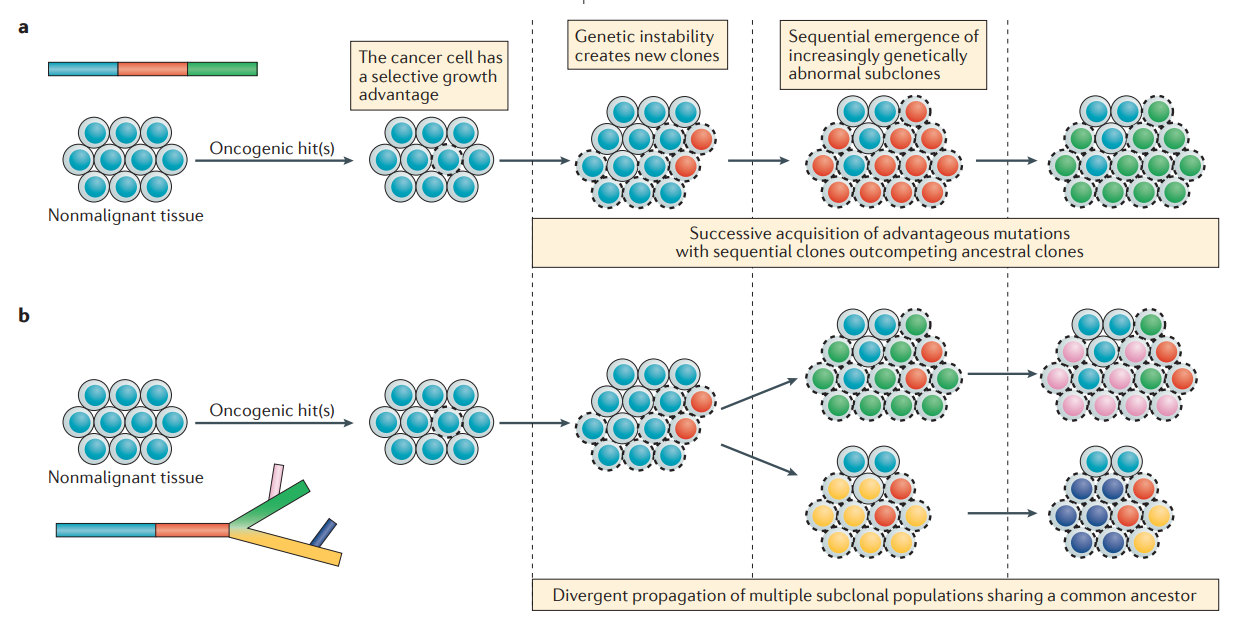
\includegraphics[width=0.9\textwidth]{image_09.PNG}
    \label{fig: tumor evolution}
  \end{figure}
  
  A \underline{\textbf{metastasis}} can either have:
  \begin{itemize}
    \item \textbf{Monoclonal origin}: meaning that it originates from tumor
    cells coming from a single lesion. In this case you have similar features as
    the starting mass and overall low heterogeneity within the metastasis.
    \item \textbf{Polyclonal origin}: meaning that it originates from multiple
    tumor cells coming from different lesions. This phenomenon is called
    \textbf{multiclonal seeding} and it leads to high lesion heterogeneity.
    Moreover, the fact that it displays some of the features from each of the
    parental lesions makes the analysis more complex.
  \end{itemize}
  
  As previously mentioned, tumor heterogeneity plays a big role in defining
  treatment resistance. We talk about two types of drug resistance (figure
  \ref{fig: tumor resistance}):
  \begin{itemize}
    \item \textbf{Primary resistance}: the pre-treatment tumor mass already
    contains cells that are resistant to the treatment; the treatment kills the
    non-resistant cells, hence the resistant clone expands. 
    \item \textbf{Acquired resistance}: the pre-treatment tumor mass does not
    already contains cells completely resistant to the treatment; the clones
    that can survive the treatment the best could then mutate in order to
    acquire a treatment immunity mechanism. 
  \end{itemize}

  \begin{figure}[H]
    \caption{Primary resistance against acquired}
    \centering
    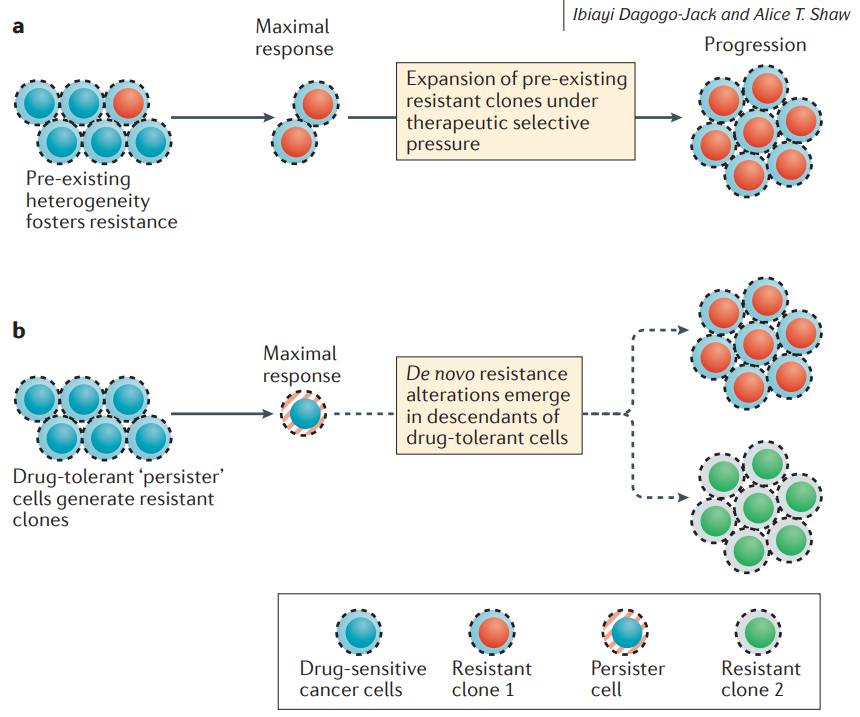
\includegraphics[width=0.6\textwidth]{image_08.PNG}
    \label{fig: tumor resistance}
  \end{figure}

  In case of primary resistance, the tumor might already display some biomarkers
  pointing to some treatment resistance; this is useful for the tumor boards in
  order to avoid needless harmful treatments. However, no biomarkers for each
  treatment are known, plus the tumor can always evolve unpredictably and
  acquire a new resistance. 


\section{Algorithms to study tumor evolution}
  
  You can study tumor evolution using information from:
  \begin{itemize}
    \item Samples from the \textbf{same subject}, from different time points or
    lesions; this way you can reconstruct mutation order and metastatic
    processes within the individual (base on shared or not mutations). 
    \item Samples from \textbf{different subjects} affected by the same
    pathology (e.g. prostate cancer); you use recurring patterns across
    individuals, this way you can reconstruct more generic features of the
    pathogenesis, for instance:
    \begin{itemize}
      \item Very common mutations in the pathology (those shared across many
      individuals)
      \item Mutations that tend to happen in a specific order (take for instance
      two mutations \textit{A} and \textit{B}; if in the majority of tumors
      which present both lesions, \textit{B} is almost always subclonal to
      \textit{A}, then probably \textit{A} tends to happen prior to \textit{B}).
    \end{itemize}
    \begin{figure}[ht]
      \caption{Tumor evolution time using samples from different individuals}
      \centering
      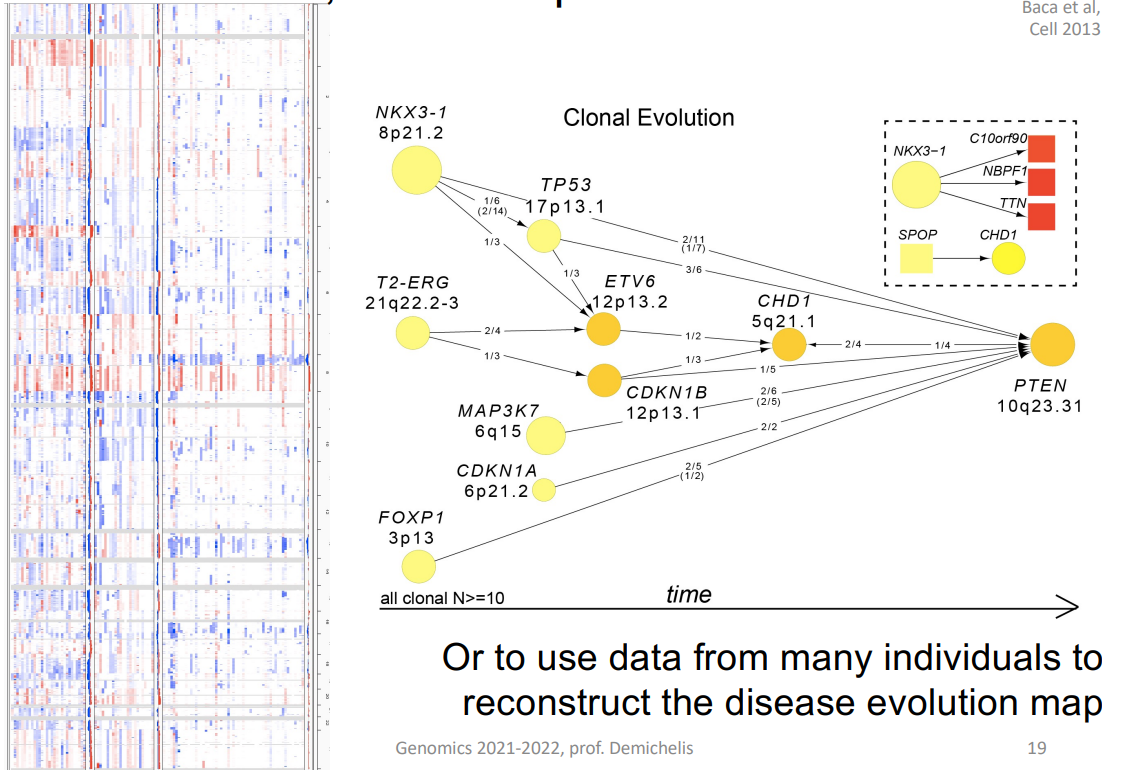
\includegraphics[width=1\textwidth]{image_10.PNG}
      \label{fig: tumor evol algorithm}
    \end{figure}
  \end{itemize}

  For more in depth reading (clickable links):
  \begin{itemize}
    \item \href{https://pubmed.ncbi.nlm.nih.gov/25830880/}{\textit{The
    evolutionary history of lethal metastatic prostate cancer, Gundem et al,
    Nature 2015}}
    \item \href{https://pubmed.ncbi.nlm.nih.gov/23622249/}{\textit{Punctuated
    evolution of prostate cancer genomes, Baca et al, Cell 2013}}
  \end{itemize}
  In general, when you have some tumor data, you try to see which of your models
  best fits the progression. \\

  There are \textit{several aspects that must be taken into account during this
  type of analysis}; most of them are useful in comprehending the pathology and
  its mechanisms, but at the same time they make analyzing the NGS data more
  difficult. Some of these aspects are: \textbf{Heterogeneity} (inter-patient,
  intra-patient, intra-tumor), \textbf{Time dependence} (tumor changes
  overtime), \textbf{Treatment status} (was the tumor treated, if yes how?),
  \textbf{Admixture DNA} (presence of non-tumoral DNA)
  
  \begin{definition}
    In a tumor biopsy you could have (and this is generally the case) other
  cells that are not tumoral (healthy tissue cells, stromal cells,
  leukocytes...). It is then defined the concept of \textbf{admixture}, which is
  \textit{the fraction of non-tumoral DNA within the sample}. Admixture is then
  used to define \textbf{tumor purity}, which is
  $$
  \text{tumor purity } = 1 - \text{ admixture}
  $$
  \end{definition}
  To sum up, a fully tumoral sample would have admixture equal to zero and
  purity equal to one. The opposite holds for healthy tissue (purity equal to
  zero, admixture equal to one). Deconvoluting the sequences derived from
  admixed DNA complicates NGS data analysis, but also provides useful
  information:
  \begin{itemize}
    \item Aggressiveness of a lesion; in general, the lower the purity, the
    better the outcome
    \item Defining whether a mutation is actually part of a subclonal tumor
    population or it is just admixed DNA
  \end{itemize}
  
  The most useful \textbf{features from NGS for characterizing tumor evolution}
  (clonality, purity and so on) are:
  \begin{itemize}
    \item Copy number mutations
    \item Point mutations
    \item Single cell sequencing
    \item Polymorphic information (which SNPs does the tumor have). The
    algorithms used to study tumor evolution use \textbf{informative SNPs},
    meaning:
    \begin{itemize}
      \item SNPs for which the individual is heterozigous (hence they vary from
      individual to individual)
      \item SNPs for which the allelic fraction is easily measurable \\
    \end{itemize}
  \end{itemize}

  
  Making \textbf{parsimonious} assumptions (mainly that all clones have the same
  growth rate), these algorithms allow to study any form of genetic aberration.
  \\

  In order to quantify the variability of tumors, it is possible to exploit the
  minor allele frequency and allelic fraction quantifications.
  \begin{itemize}
    \item \textbf{Minor allele frequency}: Minor allele frequency (MAF) is the
    frequency at which the second most common allele occurs in a given
    population.
    \item \textbf{Allelic fraction}: Proportion of reads supporting the
    alternative base.
    $$
    \text{Allelic fraction} = \frac{\text{locus reads with counted allele}}{\text{total locus reads}} 
    $$ 
    The \textbf{allelic fraction} for an informative SNP can be:
    \begin{itemize}
      \item 0 if the alternative allele was deleted
      \item 1 if the reference allele was deleted (the non-alternative one)
      \item Around 1/2 if both alleles are present in equal proportion
      \item Some other value in the range (0,1), that could be due to
      duplication, heterogeneity (admixture and/or subclonality), errors and so
      on. In this case some further information might be required (for instance
      the coverage)
    \end{itemize}

    \item \textbf{Neutral reads}: reads equally representing parental
    chromosomes. Neutral reads are quantified through Beta fraction.
    \textbf{Beta fraction}: percentage of neutral reads. Beta goes from 0 to 1;
    the closer the value to 1, the closer the reads are to a 50/50 split among
    parental sequences, the closer the value to 0, the closer the reads are to a
    100/0 split in favour of either parental sequence. The \textbf{beta
    fraction} can be:
    \begin{itemize}
      \item 0 if either allele was deleted (hence you have only one)
      \item 1 if both alleles are equally-represented (normal condition)
      \item Any other value in the range (0,1), and this is also due to
      heterogeneity and other factors.\\
    \end{itemize} 
  \end{itemize}

  \textbf{Using allele frequency and beta fraction, informative SNPs} can be
  used to reconstruct the genealogy of the mutations. If there is a deletion of
  a region then you have a \textbf{loss of heterozygosis} for all SNPs in that
  region (since you chose informative SNPs, hence heterozygous ones); then based
  on the mutations present or absent in the different clones of the lesion
  (since you do not have a perfectly homogeneous mass) you can reconstruct their
  order.  

  When designing a test you need multiple informative SNPs for each genomic
  fragment of interest. Moreover you have to choose \textbf{alleles that have
  high MAF} (hence the minor allele frequency is still rather high), since those
  are more likely to give you information. 

  For more in depth reading (clickable links):
  \begin{itemize}
    \item \href{https://pubmed.ncbi.nlm.nih.gov/31524989/}{\textit{Ploidy- and
    Purity-Adjusted Allele-Specific DNA Analysis Using CLONETv2, Davide Prandi,
    Francesca Demichelis, 2019}}
  \end{itemize}

  \begin{figure}[H]
    \caption{(A) Example of the allelic fraction (AF) and beta ($\beta$) values
    as computed in five genomic positions (p1 to pm) corresponding to five
    informative SNPs. Positions p1 to pn are within a hemizygous deleted genomic
    segment A, while genomic positions pn+1 to pm lie within a wild type genomic
    segment B. (B-D) Examples of a normal cell and two different tumor cells.
    Tumor cells 1 and 2 differ in the status of genomic segment B. Histograms
    below the cell cartoons report the expected distribution of the AF of SNPs
    in genomic segments A and B together with the associated beta values. (E-F)
    Examples of two different tumor samples. Tumor sample 1 includes one normal
    cell and nine tumor cells with deleted genomic segment A and wild type
    genomic segment B. Tumor sample 2 differs from tumor sample 1 in the
    presence of six tumor cells with a hemizygous deletion of genomic segment B.
    Expected distribution of the AF of informative SNPs together with estimated
    $\beta$ are depicted below each tumor sample cartoon.}
    \centering
    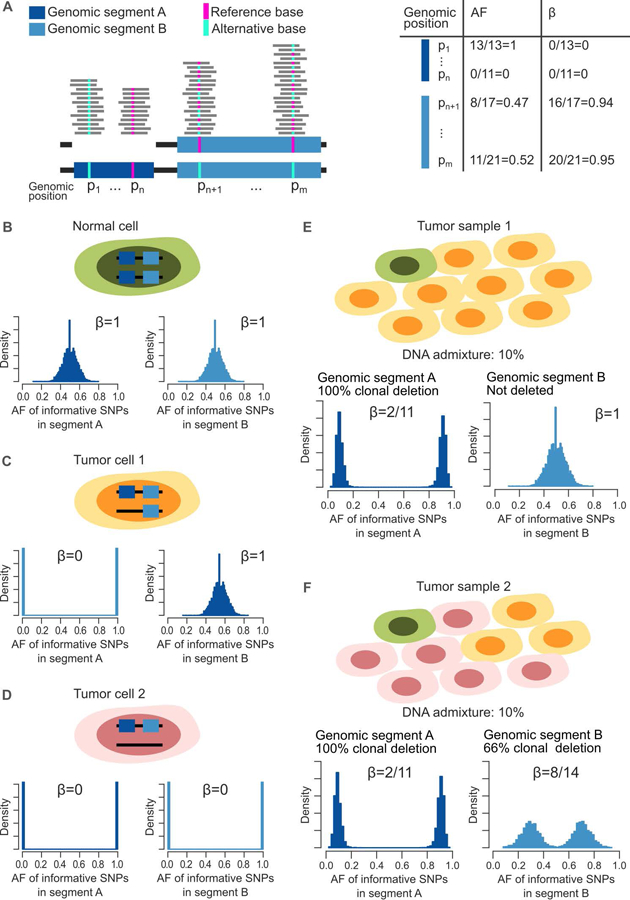
\includegraphics[width=0.7\textwidth]{image_01.jpg}
    % \label{fig: }
  \end{figure}


\section{Estimating admixture and clonality}
  Notice that the beta fraction correlates with the shape of the distribution of
  the allelic fractions of the informatives SNPs in the read;\textbf{ with
  $\beta$ = 1, you have a normal distribution with mean 0.5, with $\beta$ = 0
  you have two sharp peaks at 0 and 1, with any intermediate value you have to
  peaks which can be partially overlapping for values close to 1}. Notice that
  increasing the coverage does increase the resolution of the peaks. For this
  reason increasing the coverage (with beta constant) does increase the ability
  to distinguish clonality, especially of populations that are only some degree
  of difference from each other.
  
  \begin{figure}[H]
    \caption{As $\beta$ increases, the peaks become wider and go towards the
    center of the graph. With higher values of coverage, given the same $\beta$,
    peaks (involving the two possible variants) become more distinguished.}
    \centering
    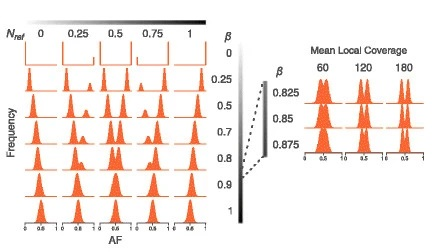
\includegraphics[width=0.75\textwidth]{image_02.jpg}
    % \label{fig: }
  \end{figure}

  To \underline{\textbf{estimate the admixture/clonality}} of a cell population:
  \begin{itemize}
    \item Measure the \textbf{allelic fraction and beta fraction of each
    informative SNP} of a genomic region
    \item For each region try which of the models \textbf{fits your data the
    best} (basically map the distribution of the allelic fractions of the region
    against prefitted reference distributions) 

    % #TODO Questo significa trovare un riferimento adeguato? in che senso?
    \item You can then compute the local and the global admixture:
    \begin{itemize}
      \item \textbf{Local admixture} (calculated on a part of the sample) is a
      measure of the fraction of cells displaying a certain lesion; for this
      reason local admixture is used as an estimate for $\rightarrow$
      \textbf{clonality}
      \item \textbf{Global admixture} is a measure of how many cells, on
      average, have a lesion; this can be used to estimate the $\rightarrow$
      \textbf{DNA admixture} (purity) of the sample
    \end{itemize}
  \end{itemize}
  Hence this technique allows you to distinguish purity and subclonality.
  
  Graphically you obtain a plot with:
  \begin{itemize}
    \item On the x axis, the cromosomal coordinates indexed by informative SNPs.
    The longer the horizontal segment, the bigger the considered region. 
    \item On the y axis, the MAF values for the informative SNPs. Any drop below
    the 0.5 value means that the region does not have a 50/50 split (in fact, a
    MAF value of $0.5$ means that the minor allele is present in 50\% of the
    reads, as the "reference" allele). The deeper the drop the deeper the
    difference in the representation of the alleles. 
  \end{itemize}

  \begin{figure}[H]
    \caption{ Top subplot: represents the MAF distribution of a clonal cell
      population. In all the local cases drops in MAF are present also in the
      reference sample; Bottom subplot: local changes in MAFs do not mirror
      properly those present in the reference sample }
    \centering
    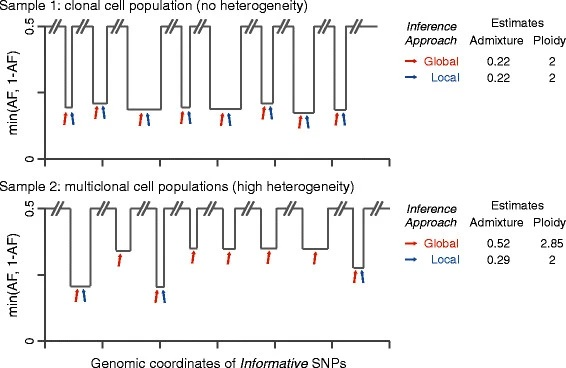
\includegraphics[width=0.9\textwidth]{image_03.jpg}
    \label{fig: local globla admixture}
  \end{figure}

  In the example picture \ref*{fig: local globla admixture}, the top subplot
  shows drops which have very similar depth, hence global and local admixtures
  are similar and there is very low heterogeneity. In the bottom subplot you
  have differences in local and global admixtures, hence we can infer the
  presence of different clonal populations. 
  
  For this type of analysis is always useful to have the \textbf{match normal
  DNA} (the non-tumor DNA of the subject): match normal DNA is usually obtained
  from leukocytes in the blood, otherwhise one could somehow deconvolute the
  signal of the admixed cells. \\

  Another graphical representation in bidimensional space is the following plot
  (figure \ref{fig: log2 plot}):
  \begin{itemize}
    \item On the x axis the \textbf{log2 ratio}, meaning 
      $$
      \text{log2 ratio} = \log_2\frac{\text{local tumor coverage}}{\text{local normal coverage}}
      $$ 
      This indicates how abundant cancer DNA is with respect to healthy DNA
      (gain of DNA if above zero, loss of DNA if below zero).
    \item On the y axis the \textbf{apparent admixture}, which is a measure of
    subclonality and is defined as
      $$
      \text{Adm. apparent} = \frac{\beta}{2 - \beta}
      $$
      Notice that this measure refers to each individual deletion/abnormality.
    \item The dots which represent the individual genomic segments. The dots
    tend to create multiple clusters and the closer two points are, the more
    probable the events they represent are close to each other in time. when
    dots are in a same cluster it means that they very likely share the same
    copy number status and also the same level of clonality.
  \end{itemize}
  
  \begin{figure}[ht]
    \caption{log2 ratio representation: when beta is equal
    to 1 the concept of admixture (1-purity) is equal to 1 meaning that purity is
    equal to 0 if we are at the top of the y scale it means that there's no signal
    related to tumor content, while the lower we go, so the closer we get to 0, the
    higher the tumor content and the level of clonality is. We have losses and
    gain of DNA copies, moving on the x axis.}
    \centering
    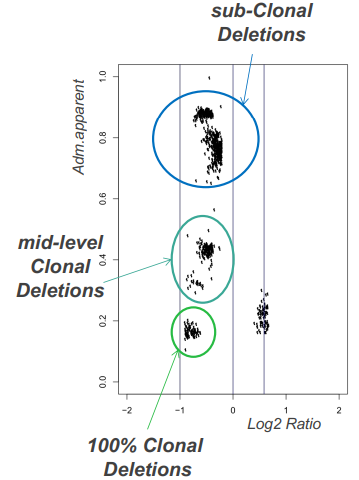
\includegraphics[width=0.6\textwidth]{image_04.png}
    \label{fig: log2 plot}
  \end{figure}
  
  You can compute clonality using the formula:
  $$
  \text{clonality} = \frac{1 - \text{Adm. apparent}}{1 - \text{Adm. global}}
  $$

  An example of how heterogeineity can lead to difficult to interpret results
  can be found in the following paper:
  \href{https://pubmed.ncbi.nlm.nih.gov/25160065/}{\textit{Unraveling the clonal
  hierarchy of somatic genomic aberrations}}. \\


